\documentclass[aspectratio=43]{beamer}
\usepackage[version=4]{mhchem}
\usepackage[skip=2pt]{caption}
\usepackage{amsmath}
\usepackage{siunitx}

% Command to display isotopes
\newcommand{\iso}[2]{\ce{^{#1}#2}}
% Set caption package options
\captionsetup{labelformat=empty}

\title[SF quenching]{Quenching of spectroscopic factors in \\ \texorpdfstring{\iso{10,12}{Be}(d, \iso{3}{He})}{10,12Be(d,3He)} reactions}
\date{Zakopane 2024 Conference}
\author[M. Lozano et al.]{M. Lozano-González, A. Matta, B. Fernández-Domínguez}
\institute{IGFAE and LPC-Caen}

\usetheme{igfae}

\begin{document}

\maketitle

\section{Motivation}
\begin{frame}{A recap on spectroscopic factors}
    \textbf{Spectroscopic factors} arise from the breakdown of the single-particle scheme to describe nuclear reactions:
    \begin{equation*}
        \sigma = C^{2}S \cdot \sigma_{s.p}
    \end{equation*}
    \begin{columns}[T]
        \begin{column}{0.48\linewidth}
            \begin{itemize}
                \item \textbf{Long-range} correlations: vibrations, giant resonances,...
                \item \textbf{Short-range}: tensor forces,...
            \end{itemize}
            \hfill{}
                \begin{beamercolorbox}[sep=1.25em, center, wd=0.75\linewidth,rounded=true]{box1}
                    Reduction of \sim\qty{65}{\percent}!
                \end{beamercolorbox}%
                \hfill{}
        \end{column}
        \begin{column}{0.48\linewidth}
            \begin{figure}
                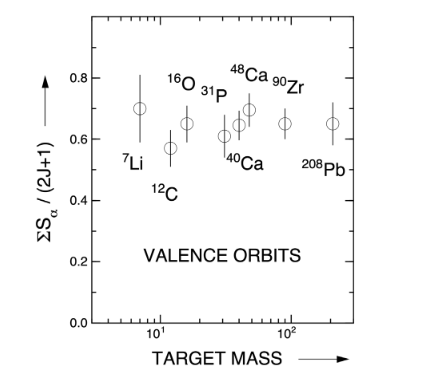
\includegraphics[width=0.9\linewidth]{figures/SF_aumann_review.png}
                \caption{T. Aumann \textit{et al.} Prog. Part. Nucl. Phys. 118 (2021)}
            \end{figure}
        \end{column}
    \end{columns}
\end{frame}

\begin{frame}{A long-standing puzzle}
    A trend with asymmetry $\Delta S \equiv S_{n} - S_{p}$ is found depending on the experimental \textbf{probe}!
    \begin{figure}
        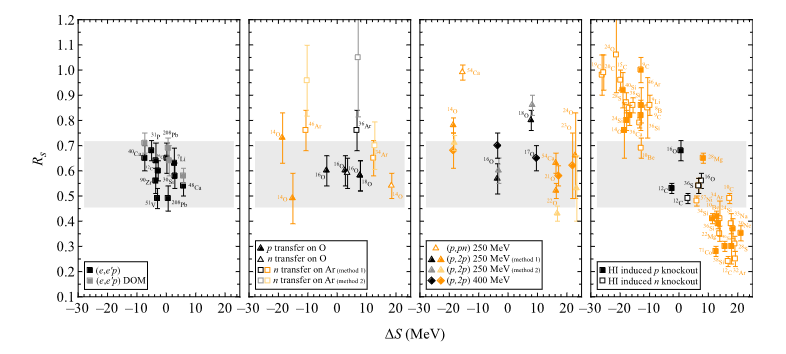
\includegraphics[width=0.9\linewidth]{figures/Rs_aumann_review.png}
        \caption{T. Aumann \textit{et al.} Prog. Part. Nucl. Phys. 118 (2021)}
    \end{figure}

\end{frame}

\begin{frame}{A longer title}
    \begin{itemize}
        \item one
        \item two
    \end{itemize}
\end{frame}

\end{document}